\chapter{Réseaux de neurones récurrents}

\section{Motivation}

Nous avons pu voir que les réseaux feedforward peuvent être utilisés afin d'appendre à prédire la sortie voulue en fonction de l'entrée du réseau. 

Néanmoins, ces réseaux sont limités à des entrées et des sorties de tailles fixes. De plus il ne peuvent gérer des réseaux présentant des cycles. On utilise alors des réseaux récurrents qui permettent un traitement plus efficace des séquences de données. On pourra ainsi faire de la prédiction et de la génération de séquence.

Dans un premier, nous verrons comment modéliser ces réseaux récurrents. Puis nous nous intéresserons à deux algorithmes d'optimisation permettant l'apprentissage des réseaux récurrents : real time recurrent learning (RTRL) et backpropagation through time (BPTT).

\section{Dépliage}

Nous avons dit précédemment qu'un réseau de neurones récurrent est un réseau possédant des cycles. Néanmoins, il est difficile d'imaginer que la valeur de sortie d'un neurone au temps $t$ dépende de la sortie de ce même neurone au temps $t$. Pour résoudre ce problème, nous allons ajouter une dimension temporelle à nos réseaux et permettre aux neurones au temps $t$ de dépendre des valeurs d'autres neurones au temps $t-1$.

Afin de mettre en évidence cette dépendance temporelle sur nos graphes, les arêtes reliant la sortie d'un neurone au temps $t-1$ à un neurone au temps $t$ vont être annotées par un carré comme sur la figure \ref{arete_retard}. On les appelera arête "retard".

\begin{figure}
\begin{center}
% Graphic for TeX using PGF
% Title: /home/pierre/Programming/pl-lstm/images/illustrations_cr/recurrent_edge.dia
% Creator: Dia v0.97.3
% CreationDate: Sun Jun 11 14:25:19 2017
% For: pierre
% \usepackage{tikz}
% The following commands are not supported in PSTricks at present
% We define them conditionally, so when they are implemented,
% this pgf file will use them.
\ifx\du\undefined
  \newlength{\du}
\fi
\setlength{\du}{15\unitlength}
\begin{tikzpicture}
\pgftransformxscale{1.000000}
\pgftransformyscale{-1.000000}
\definecolor{dialinecolor}{rgb}{0.000000, 0.000000, 0.000000}
\pgfsetstrokecolor{dialinecolor}
\definecolor{dialinecolor}{rgb}{1.000000, 1.000000, 1.000000}
\pgfsetfillcolor{dialinecolor}
\definecolor{dialinecolor}{rgb}{1.000000, 1.000000, 1.000000}
\pgfsetfillcolor{dialinecolor}
\pgfpathellipse{\pgfpoint{20.500000\du}{11.500000\du}}{\pgfpoint{1.500000\du}{0\du}}{\pgfpoint{0\du}{1.500000\du}}
\pgfusepath{fill}
\pgfsetlinewidth{0.100000\du}
\pgfsetdash{}{0pt}
\pgfsetdash{}{0pt}
\definecolor{dialinecolor}{rgb}{0.000000, 0.000000, 0.000000}
\pgfsetstrokecolor{dialinecolor}
\pgfpathellipse{\pgfpoint{20.500000\du}{11.500000\du}}{\pgfpoint{1.500000\du}{0\du}}{\pgfpoint{0\du}{1.500000\du}}
\pgfusepath{stroke}
\pgfsetlinewidth{0.100000\du}
\pgfsetdash{}{0pt}
\pgfsetdash{}{0pt}
\pgfsetmiterjoin
\pgfsetbuttcap
{
\definecolor{dialinecolor}{rgb}{0.000000, 0.000000, 0.000000}
\pgfsetfillcolor{dialinecolor}
% was here!!!
\pgfsetarrowsend{latex}
\definecolor{dialinecolor}{rgb}{0.000000, 0.000000, 0.000000}
\pgfsetstrokecolor{dialinecolor}
\pgfpathmoveto{\pgfpoint{21.560660\du}{10.439340\du}}
\pgfpathcurveto{\pgfpoint{24.000000\du}{9.500000\du}}{\pgfpoint{24.000000\du}{13.500000\du}}{\pgfpoint{21.560660\du}{12.560660\du}}
\pgfusepath{stroke}
}
\definecolor{dialinecolor}{rgb}{1.000000, 1.000000, 1.000000}
\pgfsetfillcolor{dialinecolor}
\pgfpathellipse{\pgfpoint{20.500000\du}{16.500000\du}}{\pgfpoint{1.500000\du}{0\du}}{\pgfpoint{0\du}{1.500000\du}}
\pgfusepath{fill}
\pgfsetlinewidth{0.100000\du}
\pgfsetdash{}{0pt}
\pgfsetdash{}{0pt}
\definecolor{dialinecolor}{rgb}{0.000000, 0.000000, 0.000000}
\pgfsetstrokecolor{dialinecolor}
\pgfpathellipse{\pgfpoint{20.500000\du}{16.500000\du}}{\pgfpoint{1.500000\du}{0\du}}{\pgfpoint{0\du}{1.500000\du}}
\pgfusepath{stroke}
\pgfsetlinewidth{0.100000\du}
\pgfsetdash{}{0pt}
\pgfsetdash{}{0pt}
\pgfsetbuttcap
{
\definecolor{dialinecolor}{rgb}{0.000000, 0.000000, 0.000000}
\pgfsetfillcolor{dialinecolor}
% was here!!!
\pgfsetarrowsend{latex}
\definecolor{dialinecolor}{rgb}{0.000000, 0.000000, 0.000000}
\pgfsetstrokecolor{dialinecolor}
\draw (20.500000\du,15.000000\du)--(20.500000\du,13.000000\du);
}
\pgfsetlinewidth{0.100000\du}
\pgfsetdash{}{0pt}
\pgfsetdash{}{0pt}
\pgfsetmiterjoin
\definecolor{dialinecolor}{rgb}{0.000000, 0.000000, 0.000000}
\pgfsetfillcolor{dialinecolor}
\fill (23.200000\du,11.200000\du)--(23.200000\du,11.700000\du)--(23.700000\du,11.700000\du)--(23.700000\du,11.200000\du)--cycle;
\definecolor{dialinecolor}{rgb}{0.000000, 0.000000, 0.000000}
\pgfsetstrokecolor{dialinecolor}
\draw (23.200000\du,11.200000\du)--(23.200000\du,11.700000\du)--(23.700000\du,11.700000\du)--(23.700000\du,11.200000\du)--cycle;
% setfont left to latex
\definecolor{dialinecolor}{rgb}{0.000000, 0.000000, 0.000000}
\pgfsetstrokecolor{dialinecolor}
\node at (20.500000\du,11.722500\du){$h$};
% setfont left to latex
\definecolor{dialinecolor}{rgb}{0.000000, 0.000000, 0.000000}
\pgfsetstrokecolor{dialinecolor}
\node at (20.500000\du,16.722500\du){$x$};
\end{tikzpicture}

\caption{Réseau de neurones récurrent où l'arête avec un carré signifie que le n\oe{}ud $h$ prend sa valeur au temps $t-1$ comme entrée au temps $t$.}
\label{arete_retard}
\end{center}
\end{figure}

On peut maintenant remarquer que pour une séquence $x_1, ..., x_n$ le réseau récurrent de la figure \ref{arete_retard} est équivalent au réseau feedforward de la figure \ref{reseau_deplie}.

\begin{figure}
\begin{center}
% Graphic for TeX using PGF
% Title: /home/pierre/Programming/pl-lstm/images/illustrations_cr/unfolded_graph.dia
% Creator: Dia v0.97.3
% CreationDate: Sun Jun 11 14:43:00 2017
% For: pierre
% \usepackage{tikz}
% The following commands are not supported in PSTricks at present
% We define them conditionally, so when they are implemented,
% this pgf file will use them.
\ifx\du\undefined
  \newlength{\du}
\fi
\setlength{\du}{15\unitlength}
\begin{tikzpicture}
\pgftransformxscale{1.000000}
\pgftransformyscale{-1.000000}
\definecolor{dialinecolor}{rgb}{0.000000, 0.000000, 0.000000}
\pgfsetstrokecolor{dialinecolor}
\definecolor{dialinecolor}{rgb}{1.000000, 1.000000, 1.000000}
\pgfsetfillcolor{dialinecolor}
\definecolor{dialinecolor}{rgb}{1.000000, 1.000000, 1.000000}
\pgfsetfillcolor{dialinecolor}
\pgfpathellipse{\pgfpoint{20.500000\du}{11.500000\du}}{\pgfpoint{1.500000\du}{0\du}}{\pgfpoint{0\du}{1.500000\du}}
\pgfusepath{fill}
\pgfsetlinewidth{0.100000\du}
\pgfsetdash{}{0pt}
\pgfsetdash{}{0pt}
\definecolor{dialinecolor}{rgb}{0.000000, 0.000000, 0.000000}
\pgfsetstrokecolor{dialinecolor}
\pgfpathellipse{\pgfpoint{20.500000\du}{11.500000\du}}{\pgfpoint{1.500000\du}{0\du}}{\pgfpoint{0\du}{1.500000\du}}
\pgfusepath{stroke}
\definecolor{dialinecolor}{rgb}{1.000000, 1.000000, 1.000000}
\pgfsetfillcolor{dialinecolor}
\pgfpathellipse{\pgfpoint{20.500000\du}{16.500000\du}}{\pgfpoint{1.500000\du}{0\du}}{\pgfpoint{0\du}{1.500000\du}}
\pgfusepath{fill}
\pgfsetlinewidth{0.100000\du}
\pgfsetdash{}{0pt}
\pgfsetdash{}{0pt}
\definecolor{dialinecolor}{rgb}{0.000000, 0.000000, 0.000000}
\pgfsetstrokecolor{dialinecolor}
\pgfpathellipse{\pgfpoint{20.500000\du}{16.500000\du}}{\pgfpoint{1.500000\du}{0\du}}{\pgfpoint{0\du}{1.500000\du}}
\pgfusepath{stroke}
\pgfsetlinewidth{0.100000\du}
\pgfsetdash{}{0pt}
\pgfsetdash{}{0pt}
\pgfsetbuttcap
{
\definecolor{dialinecolor}{rgb}{0.000000, 0.000000, 0.000000}
\pgfsetfillcolor{dialinecolor}
% was here!!!
\pgfsetarrowsend{latex}
\definecolor{dialinecolor}{rgb}{0.000000, 0.000000, 0.000000}
\pgfsetstrokecolor{dialinecolor}
\draw (20.500000\du,15.000000\du)--(20.500000\du,13.000000\du);
}
% setfont left to latex
\definecolor{dialinecolor}{rgb}{0.000000, 0.000000, 0.000000}
\pgfsetstrokecolor{dialinecolor}
\node at (20.500000\du,11.722500\du){$h(1)$};
% setfont left to latex
\definecolor{dialinecolor}{rgb}{0.000000, 0.000000, 0.000000}
\pgfsetstrokecolor{dialinecolor}
\node at (20.500000\du,16.722500\du){$x_1$};
\definecolor{dialinecolor}{rgb}{1.000000, 1.000000, 1.000000}
\pgfsetfillcolor{dialinecolor}
\pgfpathellipse{\pgfpoint{25.500000\du}{11.500000\du}}{\pgfpoint{1.500000\du}{0\du}}{\pgfpoint{0\du}{1.500000\du}}
\pgfusepath{fill}
\pgfsetlinewidth{0.100000\du}
\pgfsetdash{}{0pt}
\pgfsetdash{}{0pt}
\definecolor{dialinecolor}{rgb}{0.000000, 0.000000, 0.000000}
\pgfsetstrokecolor{dialinecolor}
\pgfpathellipse{\pgfpoint{25.500000\du}{11.500000\du}}{\pgfpoint{1.500000\du}{0\du}}{\pgfpoint{0\du}{1.500000\du}}
\pgfusepath{stroke}
\definecolor{dialinecolor}{rgb}{1.000000, 1.000000, 1.000000}
\pgfsetfillcolor{dialinecolor}
\pgfpathellipse{\pgfpoint{25.500000\du}{16.500000\du}}{\pgfpoint{1.500000\du}{0\du}}{\pgfpoint{0\du}{1.500000\du}}
\pgfusepath{fill}
\pgfsetlinewidth{0.100000\du}
\pgfsetdash{}{0pt}
\pgfsetdash{}{0pt}
\definecolor{dialinecolor}{rgb}{0.000000, 0.000000, 0.000000}
\pgfsetstrokecolor{dialinecolor}
\pgfpathellipse{\pgfpoint{25.500000\du}{16.500000\du}}{\pgfpoint{1.500000\du}{0\du}}{\pgfpoint{0\du}{1.500000\du}}
\pgfusepath{stroke}
\pgfsetlinewidth{0.100000\du}
\pgfsetdash{}{0pt}
\pgfsetdash{}{0pt}
\pgfsetbuttcap
{
\definecolor{dialinecolor}{rgb}{0.000000, 0.000000, 0.000000}
\pgfsetfillcolor{dialinecolor}
% was here!!!
\pgfsetarrowsend{latex}
\definecolor{dialinecolor}{rgb}{0.000000, 0.000000, 0.000000}
\pgfsetstrokecolor{dialinecolor}
\draw (25.500000\du,15.000000\du)--(25.500000\du,13.000000\du);
}
\definecolor{dialinecolor}{rgb}{1.000000, 1.000000, 1.000000}
\pgfsetfillcolor{dialinecolor}
\pgfpathellipse{\pgfpoint{34.500000\du}{11.500000\du}}{\pgfpoint{1.500000\du}{0\du}}{\pgfpoint{0\du}{1.500000\du}}
\pgfusepath{fill}
\pgfsetlinewidth{0.100000\du}
\pgfsetdash{}{0pt}
\pgfsetdash{}{0pt}
\definecolor{dialinecolor}{rgb}{0.000000, 0.000000, 0.000000}
\pgfsetstrokecolor{dialinecolor}
\pgfpathellipse{\pgfpoint{34.500000\du}{11.500000\du}}{\pgfpoint{1.500000\du}{0\du}}{\pgfpoint{0\du}{1.500000\du}}
\pgfusepath{stroke}
\definecolor{dialinecolor}{rgb}{1.000000, 1.000000, 1.000000}
\pgfsetfillcolor{dialinecolor}
\pgfpathellipse{\pgfpoint{34.500000\du}{16.500000\du}}{\pgfpoint{1.500000\du}{0\du}}{\pgfpoint{0\du}{1.500000\du}}
\pgfusepath{fill}
\pgfsetlinewidth{0.100000\du}
\pgfsetdash{}{0pt}
\pgfsetdash{}{0pt}
\definecolor{dialinecolor}{rgb}{0.000000, 0.000000, 0.000000}
\pgfsetstrokecolor{dialinecolor}
\pgfpathellipse{\pgfpoint{34.500000\du}{16.500000\du}}{\pgfpoint{1.500000\du}{0\du}}{\pgfpoint{0\du}{1.500000\du}}
\pgfusepath{stroke}
\pgfsetlinewidth{0.100000\du}
\pgfsetdash{}{0pt}
\pgfsetdash{}{0pt}
\pgfsetbuttcap
{
\definecolor{dialinecolor}{rgb}{0.000000, 0.000000, 0.000000}
\pgfsetfillcolor{dialinecolor}
% was here!!!
\pgfsetarrowsend{latex}
\definecolor{dialinecolor}{rgb}{0.000000, 0.000000, 0.000000}
\pgfsetstrokecolor{dialinecolor}
\draw (34.500000\du,15.000000\du)--(34.500000\du,13.000000\du);
}
\pgfsetlinewidth{0.100000\du}
\pgfsetdash{}{0pt}
\pgfsetdash{}{0pt}
\pgfsetbuttcap
{
\definecolor{dialinecolor}{rgb}{0.000000, 0.000000, 0.000000}
\pgfsetfillcolor{dialinecolor}
% was here!!!
\pgfsetarrowsend{latex}
\definecolor{dialinecolor}{rgb}{0.000000, 0.000000, 0.000000}
\pgfsetstrokecolor{dialinecolor}
\draw (22.000000\du,11.500000\du)--(23.950806\du,11.500000\du);
}
\definecolor{dialinecolor}{rgb}{1.000000, 1.000000, 1.000000}
\pgfsetfillcolor{dialinecolor}
\pgfpathellipse{\pgfpoint{39.500000\du}{11.500000\du}}{\pgfpoint{1.500000\du}{0\du}}{\pgfpoint{0\du}{1.500000\du}}
\pgfusepath{fill}
\pgfsetlinewidth{0.100000\du}
\pgfsetdash{}{0pt}
\pgfsetdash{}{0pt}
\definecolor{dialinecolor}{rgb}{0.000000, 0.000000, 0.000000}
\pgfsetstrokecolor{dialinecolor}
\pgfpathellipse{\pgfpoint{39.500000\du}{11.500000\du}}{\pgfpoint{1.500000\du}{0\du}}{\pgfpoint{0\du}{1.500000\du}}
\pgfusepath{stroke}
\definecolor{dialinecolor}{rgb}{1.000000, 1.000000, 1.000000}
\pgfsetfillcolor{dialinecolor}
\pgfpathellipse{\pgfpoint{39.500000\du}{16.500000\du}}{\pgfpoint{1.500000\du}{0\du}}{\pgfpoint{0\du}{1.500000\du}}
\pgfusepath{fill}
\pgfsetlinewidth{0.100000\du}
\pgfsetdash{}{0pt}
\pgfsetdash{}{0pt}
\definecolor{dialinecolor}{rgb}{0.000000, 0.000000, 0.000000}
\pgfsetstrokecolor{dialinecolor}
\pgfpathellipse{\pgfpoint{39.500000\du}{16.500000\du}}{\pgfpoint{1.500000\du}{0\du}}{\pgfpoint{0\du}{1.500000\du}}
\pgfusepath{stroke}
\pgfsetlinewidth{0.100000\du}
\pgfsetdash{}{0pt}
\pgfsetdash{}{0pt}
\pgfsetbuttcap
{
\definecolor{dialinecolor}{rgb}{0.000000, 0.000000, 0.000000}
\pgfsetfillcolor{dialinecolor}
% was here!!!
\pgfsetarrowsend{latex}
\definecolor{dialinecolor}{rgb}{0.000000, 0.000000, 0.000000}
\pgfsetstrokecolor{dialinecolor}
\draw (39.500000\du,15.000000\du)--(39.500000\du,13.000000\du);
}
\pgfsetlinewidth{0.100000\du}
\pgfsetdash{}{0pt}
\pgfsetdash{}{0pt}
\pgfsetbuttcap
{
\definecolor{dialinecolor}{rgb}{0.000000, 0.000000, 0.000000}
\pgfsetfillcolor{dialinecolor}
% was here!!!
\pgfsetarrowsend{latex}
\definecolor{dialinecolor}{rgb}{0.000000, 0.000000, 0.000000}
\pgfsetstrokecolor{dialinecolor}
\draw (36.000000\du,11.500000\du)--(37.950806\du,11.500000\du);
}
% setfont left to latex
\definecolor{dialinecolor}{rgb}{0.000000, 0.000000, 0.000000}
\pgfsetstrokecolor{dialinecolor}
\node at (25.500000\du,16.722500\du){$x_2$};
% setfont left to latex
\definecolor{dialinecolor}{rgb}{0.000000, 0.000000, 0.000000}
\pgfsetstrokecolor{dialinecolor}
\node at (34.500000\du,16.722500\du){$x_{n-1}$};
% setfont left to latex
\definecolor{dialinecolor}{rgb}{0.000000, 0.000000, 0.000000}
\pgfsetstrokecolor{dialinecolor}
\node at (39.500000\du,16.722500\du){$x_n$};
% setfont left to latex
\definecolor{dialinecolor}{rgb}{0.000000, 0.000000, 0.000000}
\pgfsetstrokecolor{dialinecolor}
\node at (25.500000\du,11.722500\du){$h(2)$};
% setfont left to latex
\definecolor{dialinecolor}{rgb}{0.000000, 0.000000, 0.000000}
\pgfsetstrokecolor{dialinecolor}
\node at (34.500000\du,11.722500\du){$h(n-1)$};
% setfont left to latex
\definecolor{dialinecolor}{rgb}{0.000000, 0.000000, 0.000000}
\pgfsetstrokecolor{dialinecolor}
\node at (39.500000\du,11.722500\du){$h(n)$};
\pgfsetlinewidth{0.100000\du}
\pgfsetdash{}{0pt}
\pgfsetdash{}{0pt}
\pgfsetbuttcap
{
\definecolor{dialinecolor}{rgb}{0.000000, 0.000000, 0.000000}
\pgfsetfillcolor{dialinecolor}
% was here!!!
\pgfsetarrowsend{latex}
\definecolor{dialinecolor}{rgb}{0.000000, 0.000000, 0.000000}
\pgfsetstrokecolor{dialinecolor}
\draw (27.000000\du,11.500000\du)--(29.000000\du,11.500000\du);
}
\pgfsetlinewidth{0.100000\du}
\pgfsetdash{}{0pt}
\pgfsetdash{}{0pt}
\pgfsetbuttcap
{
\definecolor{dialinecolor}{rgb}{0.000000, 0.000000, 0.000000}
\pgfsetfillcolor{dialinecolor}
% was here!!!
\pgfsetarrowsend{latex}
\definecolor{dialinecolor}{rgb}{0.000000, 0.000000, 0.000000}
\pgfsetstrokecolor{dialinecolor}
\draw (31.000000\du,11.500000\du)--(33.000000\du,11.500000\du);
}
% setfont left to latex
\definecolor{dialinecolor}{rgb}{0.000000, 0.000000, 0.000000}
\pgfsetstrokecolor{dialinecolor}
\node at (30.000000\du,11.722500\du){$...$};
% setfont left to latex
\definecolor{dialinecolor}{rgb}{0.000000, 0.000000, 0.000000}
\pgfsetstrokecolor{dialinecolor}
\node at (20.500000\du,8.722500\du){$t=1$};
% setfont left to latex
\definecolor{dialinecolor}{rgb}{0.000000, 0.000000, 0.000000}
\pgfsetstrokecolor{dialinecolor}
\node at (25.500000\du,8.722500\du){$t=2$};
% setfont left to latex
\definecolor{dialinecolor}{rgb}{0.000000, 0.000000, 0.000000}
\pgfsetstrokecolor{dialinecolor}
\node at (34.500000\du,8.722500\du){$t=n-1$};
% setfont left to latex
\definecolor{dialinecolor}{rgb}{0.000000, 0.000000, 0.000000}
\pgfsetstrokecolor{dialinecolor}
\node at (39.500000\du,8.722500\du){$t=n$};
\end{tikzpicture}

\caption{Réseau de neurones feedforward équivalent au réseau récurrent de la figure \ref{arete_retard} pour la séquence d'entrée $x_1, ..., x_n$.}
\label{reseau_deplie}
\end{center}
\end{figure}

Le processus de passage d'un réseau récurrent à un réseau feedforward s'appelle dépliage.

Une fois le réseau déplié obtenu, on peut utiliser l'algorithme de propagation classique pour les graphes de calculs afin de calculer la sortie du réseau récurrent.

Nous avons utilisé trois méthodes pour générer des réseaux dépliés. La première prend en entrée un réseau récurrent avec des arêtes retards et obtient le dépliage à partir de celui-ci.

La seconde prend en entrée un \textit{layer}, représenté figure \ref{layer}, c'est-à-dire le sous-graphe qui va être copié à chaque pas de temps et le clone autant de fois qu'il le faut.

\begin{figure}
\begin{center}
% Graphic for TeX using PGF
% Title: /home/pierre/Programming/pl-lstm/images/illustrations_cr/layer.dia
% Creator: Dia v0.97.3
% CreationDate: Wed Mar  8 22:39:59 2017
% For: pierre
% \usepackage{tikz}
% The following commands are not supported in PSTricks at present
% We define them conditionally, so when they are implemented,
% this pgf file will use them.
\ifx\du\undefined
  \newlength{\du}
\fi
\setlength{\du}{15\unitlength}
\begin{tikzpicture}[scale=0.5]
\pgftransformxscale{1.000000}
\pgftransformyscale{-1.000000}
\definecolor{dialinecolor}{rgb}{0.000000, 0.000000, 0.000000}
\pgfsetstrokecolor{dialinecolor}
\definecolor{dialinecolor}{rgb}{1.000000, 1.000000, 1.000000}
\pgfsetfillcolor{dialinecolor}
\pgfsetlinewidth{0.100000\du}
\pgfsetdash{}{0pt}
\pgfsetdash{}{0pt}
\pgfsetmiterjoin
\definecolor{dialinecolor}{rgb}{1.000000, 1.000000, 1.000000}
\pgfsetfillcolor{dialinecolor}
\fill (12.105000\du,6.867500\du)--(12.105000\du,21.867500\du)--(22.105000\du,21.867500\du)--(22.105000\du,6.867500\du)--cycle;
\definecolor{dialinecolor}{rgb}{0.000000, 0.000000, 0.000000}
\pgfsetstrokecolor{dialinecolor}
\draw (12.105000\du,6.867500\du)--(12.105000\du,21.867500\du)--(22.105000\du,21.867500\du)--(22.105000\du,6.867500\du)--cycle;
\pgfsetlinewidth{0.100000\du}
\pgfsetdash{}{0pt}
\pgfsetdash{}{0pt}
\pgfsetbuttcap
{
\definecolor{dialinecolor}{rgb}{0.000000, 0.000000, 0.000000}
\pgfsetfillcolor{dialinecolor}
% was here!!!
\pgfsetarrowsend{latex}
\definecolor{dialinecolor}{rgb}{0.000000, 0.000000, 0.000000}
\pgfsetstrokecolor{dialinecolor}
\draw (17.105000\du,24.867500\du)--(17.105000\du,21.867500\du);
}
\pgfsetlinewidth{0.100000\du}
\pgfsetdash{}{0pt}
\pgfsetdash{}{0pt}
\pgfsetbuttcap
{
\definecolor{dialinecolor}{rgb}{0.000000, 0.000000, 0.000000}
\pgfsetfillcolor{dialinecolor}
% was here!!!
\pgfsetarrowsend{latex}
\definecolor{dialinecolor}{rgb}{0.000000, 0.000000, 0.000000}
\pgfsetstrokecolor{dialinecolor}
\draw (17.105000\du,3.867500\du)--(17.105000\du,6.867500\du);
}
\pgfsetlinewidth{0.100000\du}
\pgfsetdash{}{0pt}
\pgfsetdash{}{0pt}
\pgfsetbuttcap
{
\definecolor{dialinecolor}{rgb}{0.301961, 0.301961, 0.301961}
\pgfsetfillcolor{dialinecolor}
% was here!!!
\pgfsetarrowsend{latex}
\definecolor{dialinecolor}{rgb}{0.301961, 0.301961, 0.301961}
\pgfsetstrokecolor{dialinecolor}
\draw (12.105000\du,13.867500\du)--(8.105000\du,13.867500\du);
}
% setfont left to latex
\definecolor{dialinecolor}{rgb}{0.000000, 0.000000, 0.000000}
\pgfsetstrokecolor{dialinecolor}
\node[anchor=west] at (6.000000\du,13.000000\du){$h_{in}$};
% setfont left to latex
\definecolor{dialinecolor}{rgb}{0.000000, 0.000000, 0.000000}
\pgfsetstrokecolor{dialinecolor}
\node[anchor=west] at (26.305000\du,13.067500\du){$h_{out}$};
% setfont left to latex
\definecolor{dialinecolor}{rgb}{0.301961, 0.301961, 0.301961}
\pgfsetstrokecolor{dialinecolor}
\node[anchor=west] at (5.000000\du,15.000000\du){$\frac{\partial E}{\partial h_{in}}$};
% setfont left to latex
\definecolor{dialinecolor}{rgb}{0.301961, 0.301961, 0.301961}
\pgfsetstrokecolor{dialinecolor}
\node[anchor=west] at (26.305000\du,15.067500\du){$\frac{\partial E}{\partial h_{out}}$};
\pgfsetlinewidth{0.100000\du}
\pgfsetdash{}{0pt}
\pgfsetdash{}{0pt}
\pgfsetbuttcap
{
\definecolor{dialinecolor}{rgb}{0.000000, 0.000000, 0.000000}
\pgfsetfillcolor{dialinecolor}
% was here!!!
\pgfsetarrowsend{latex}
\definecolor{dialinecolor}{rgb}{0.000000, 0.000000, 0.000000}
\pgfsetstrokecolor{dialinecolor}
\draw (8.105000\du,12.867500\du)--(12.105000\du,12.867500\du);
}
\pgfsetlinewidth{0.100000\du}
\pgfsetdash{}{0pt}
\pgfsetdash{}{0pt}
\pgfsetbuttcap
{
\definecolor{dialinecolor}{rgb}{0.301961, 0.301961, 0.301961}
\pgfsetfillcolor{dialinecolor}
% was here!!!
\pgfsetarrowsend{latex}
\definecolor{dialinecolor}{rgb}{0.301961, 0.301961, 0.301961}
\pgfsetstrokecolor{dialinecolor}
\draw (26.105000\du,13.867500\du)--(22.105000\du,13.867500\du);
}
\pgfsetlinewidth{0.100000\du}
\pgfsetdash{}{0pt}
\pgfsetdash{}{0pt}
\pgfsetbuttcap
{
\definecolor{dialinecolor}{rgb}{0.000000, 0.000000, 0.000000}
\pgfsetfillcolor{dialinecolor}
% was here!!!
\pgfsetarrowsend{latex}
\definecolor{dialinecolor}{rgb}{0.000000, 0.000000, 0.000000}
\pgfsetstrokecolor{dialinecolor}
\draw (22.105000\du,12.867500\du)--(26.105000\du,12.867500\du);
}
% setfont left to latex
\definecolor{dialinecolor}{rgb}{0.000000, 0.000000, 0.000000}
\pgfsetstrokecolor{dialinecolor}
\node at (17.105000\du,25.590000\du){$x_t$};
% setfont left to latex
\definecolor{dialinecolor}{rgb}{0.000000, 0.000000, 0.000000}
\pgfsetstrokecolor{dialinecolor}
\node at (17.000000\du,3.222500\du){$y_t$};
\end{tikzpicture}

\caption{Représentation d'un layer. Il contient les n\oe{}uds du graphe à un temps $t$. Il prend en entrée la sortie de l'état caché du temps $t-1$ appelée $h_{in}$ et l'entrée $x_t$. Il a comme sortie l'état caché $h_{out}$ ainsi que $\hat{y}_t$ qui sera comparé avec $y_t$ la sortie attendue au temps $t$. Le $layer$ sert aussi lors de la phase de rétropropagation.}
\label{layer}
\end{center}
\end{figure}

Enfin la dernière méthode est de ne pas utiliser d'algorithme "général" permettant de passer d'un graphe récurrent à un graphe acyclique. Mais plutôt d'écrire pour chaque architecture de réseau une fonction dépliant ce réseau. Une telle fonction contiendra principalement une boucle créant les n\oe{}uds nécessaires pour chaque temps.

Devant la diversité des architectures des réseaux récurrents, la dernière méthode est la plus sensée et la plus pratique. Elle offre une liberté totale quant à l'architecture du graphe tout en étant relativement simple.

\section{BPTT}

Contrairement, à ce que nous avons fait lors du projet, nous allons d'abord présenter l'algorithme \textit{backpropagation through time} (BPTT) car il s'agit d'une simple généralisation de la rétropropagation déjà présentée pour les réseaux feedforward.

L'algorithme consiste en deux étapes :
\begin{enumerate}
\item Déplier le réseau récurrent pour avoir un réseau feedforward.
\item Appliquer l'algorithme de rétropropagation à ce réseau feedforward.
\end{enumerate}

La seule difficulté conceptuelle réside donc dans le dépliage.

En pratique, le dépliage est un processus coûteux en temps. Lors de l'apprentissage, on évite donc de déplier un graphe pour chaque exemple d'apprentissage. Pour cela, si cela est possible, on fixe la taille des séquences d'entrée lors de l'apprentissage. Nous pourrons ainsi utiliser le même réseau pour tous les exemples. En outre, comme tous les exemples auront la même taille, nous pourrons les placer dans une matrice comme pour les réseaux feedforward et passer un batch d'exemples en même temps ce qui permet d'accélérer encore les calculs en utilisant pleinement la puissance de \texttt{numpy}.

\section{RTRL}

Détaillons maintenant l'algorithme RTRL qui a une philosophique complètement différente. Au lieu de rétropropager le gradient, nous allons le propager.

Nous nous plaçons dans le cas particulier où le réseau est fully connected comme sur la figure \ref{fully_connected_recurrent_network}. 

\begin{figure}
\begin{center}
% Graphic for TeX using PGF
% Title: /home/pierre/Programming/pl-lstm/images/illustrations_cr/fully_connected_recurrent_network.dia
% Creator: Dia v0.97.3
% CreationDate: Sun Jun 11 17:28:43 2017
% For: pierre
% \usepackage{tikz}
% The following commands are not supported in PSTricks at present
% We define them conditionally, so when they are implemented,
% this pgf file will use them.
\ifx\du\undefined
  \newlength{\du}
\fi
\setlength{\du}{15\unitlength}
\begin{tikzpicture}
\pgftransformxscale{1.000000}
\pgftransformyscale{-1.000000}
\definecolor{dialinecolor}{rgb}{0.000000, 0.000000, 0.000000}
\pgfsetstrokecolor{dialinecolor}
\definecolor{dialinecolor}{rgb}{1.000000, 1.000000, 1.000000}
\pgfsetfillcolor{dialinecolor}
\definecolor{dialinecolor}{rgb}{1.000000, 1.000000, 1.000000}
\pgfsetfillcolor{dialinecolor}
\pgfpathellipse{\pgfpoint{20.500000\du}{17.500000\du}}{\pgfpoint{1.500000\du}{0\du}}{\pgfpoint{0\du}{1.500000\du}}
\pgfusepath{fill}
\pgfsetlinewidth{0.100000\du}
\pgfsetdash{}{0pt}
\pgfsetdash{}{0pt}
\definecolor{dialinecolor}{rgb}{0.000000, 0.000000, 0.000000}
\pgfsetstrokecolor{dialinecolor}
\pgfpathellipse{\pgfpoint{20.500000\du}{17.500000\du}}{\pgfpoint{1.500000\du}{0\du}}{\pgfpoint{0\du}{1.500000\du}}
\pgfusepath{stroke}
\definecolor{dialinecolor}{rgb}{1.000000, 1.000000, 1.000000}
\pgfsetfillcolor{dialinecolor}
\pgfpathellipse{\pgfpoint{23.500000\du}{5.500000\du}}{\pgfpoint{1.500000\du}{0\du}}{\pgfpoint{0\du}{1.500000\du}}
\pgfusepath{fill}
\pgfsetlinewidth{0.100000\du}
\pgfsetdash{}{0pt}
\pgfsetdash{}{0pt}
\definecolor{dialinecolor}{rgb}{0.000000, 0.000000, 0.000000}
\pgfsetstrokecolor{dialinecolor}
\pgfpathellipse{\pgfpoint{23.500000\du}{5.500000\du}}{\pgfpoint{1.500000\du}{0\du}}{\pgfpoint{0\du}{1.500000\du}}
\pgfusepath{stroke}
\definecolor{dialinecolor}{rgb}{1.000000, 1.000000, 1.000000}
\pgfsetfillcolor{dialinecolor}
\pgfpathellipse{\pgfpoint{29.500000\du}{11.500000\du}}{\pgfpoint{1.500000\du}{0\du}}{\pgfpoint{0\du}{1.500000\du}}
\pgfusepath{fill}
\pgfsetlinewidth{0.100000\du}
\pgfsetdash{}{0pt}
\pgfsetdash{}{0pt}
\definecolor{dialinecolor}{rgb}{0.000000, 0.000000, 0.000000}
\pgfsetstrokecolor{dialinecolor}
\pgfpathellipse{\pgfpoint{29.500000\du}{11.500000\du}}{\pgfpoint{1.500000\du}{0\du}}{\pgfpoint{0\du}{1.500000\du}}
\pgfusepath{stroke}
\definecolor{dialinecolor}{rgb}{1.000000, 1.000000, 1.000000}
\pgfsetfillcolor{dialinecolor}
\pgfpathellipse{\pgfpoint{26.500000\du}{17.500000\du}}{\pgfpoint{1.500000\du}{0\du}}{\pgfpoint{0\du}{1.500000\du}}
\pgfusepath{fill}
\pgfsetlinewidth{0.100000\du}
\pgfsetdash{}{0pt}
\pgfsetdash{}{0pt}
\definecolor{dialinecolor}{rgb}{0.000000, 0.000000, 0.000000}
\pgfsetstrokecolor{dialinecolor}
\pgfpathellipse{\pgfpoint{26.500000\du}{17.500000\du}}{\pgfpoint{1.500000\du}{0\du}}{\pgfpoint{0\du}{1.500000\du}}
\pgfusepath{stroke}
\definecolor{dialinecolor}{rgb}{1.000000, 1.000000, 1.000000}
\pgfsetfillcolor{dialinecolor}
\pgfpathellipse{\pgfpoint{17.500000\du}{11.500000\du}}{\pgfpoint{1.500000\du}{0\du}}{\pgfpoint{0\du}{1.500000\du}}
\pgfusepath{fill}
\pgfsetlinewidth{0.100000\du}
\pgfsetdash{}{0pt}
\pgfsetdash{}{0pt}
\definecolor{dialinecolor}{rgb}{0.000000, 0.000000, 0.000000}
\pgfsetstrokecolor{dialinecolor}
\pgfpathellipse{\pgfpoint{17.500000\du}{11.500000\du}}{\pgfpoint{1.500000\du}{0\du}}{\pgfpoint{0\du}{1.500000\du}}
\pgfusepath{stroke}
\pgfsetlinewidth{0.100000\du}
\pgfsetdash{}{0pt}
\pgfsetdash{}{0pt}
\pgfsetbuttcap
{
\definecolor{dialinecolor}{rgb}{0.000000, 0.000000, 0.000000}
\pgfsetfillcolor{dialinecolor}
% was here!!!
\pgfsetarrowsend{latex}
\definecolor{dialinecolor}{rgb}{0.000000, 0.000000, 0.000000}
\pgfsetstrokecolor{dialinecolor}
\draw (19.806763\du,16.113525\du)--(18.193237\du,12.886475\du);
}
\pgfsetlinewidth{0.100000\du}
\pgfsetdash{}{0pt}
\pgfsetdash{}{0pt}
\pgfsetbuttcap
{
\definecolor{dialinecolor}{rgb}{0.000000, 0.000000, 0.000000}
\pgfsetfillcolor{dialinecolor}
% was here!!!
\pgfsetarrowsend{latex}
\definecolor{dialinecolor}{rgb}{0.000000, 0.000000, 0.000000}
\pgfsetstrokecolor{dialinecolor}
\draw (20.875916\du,15.996338\du)--(23.124084\du,7.003662\du);
}
\pgfsetlinewidth{0.100000\du}
\pgfsetdash{}{0pt}
\pgfsetdash{}{0pt}
\pgfsetbuttcap
{
\definecolor{dialinecolor}{rgb}{0.000000, 0.000000, 0.000000}
\pgfsetfillcolor{dialinecolor}
% was here!!!
\pgfsetarrowsend{latex}
\definecolor{dialinecolor}{rgb}{0.000000, 0.000000, 0.000000}
\pgfsetstrokecolor{dialinecolor}
\draw (21.788696\du,16.640869\du)--(28.211304\du,12.359131\du);
}
\pgfsetlinewidth{0.100000\du}
\pgfsetdash{}{0pt}
\pgfsetdash{}{0pt}
\pgfsetbuttcap
{
\definecolor{dialinecolor}{rgb}{0.000000, 0.000000, 0.000000}
\pgfsetfillcolor{dialinecolor}
% was here!!!
\pgfsetarrowsend{latex}
\definecolor{dialinecolor}{rgb}{0.000000, 0.000000, 0.000000}
\pgfsetstrokecolor{dialinecolor}
\draw (25.211304\du,16.640869\du)--(18.788696\du,12.359131\du);
}
\pgfsetlinewidth{0.100000\du}
\pgfsetdash{}{0pt}
\pgfsetdash{}{0pt}
\pgfsetbuttcap
{
\definecolor{dialinecolor}{rgb}{0.000000, 0.000000, 0.000000}
\pgfsetfillcolor{dialinecolor}
% was here!!!
\pgfsetarrowsend{latex}
\definecolor{dialinecolor}{rgb}{0.000000, 0.000000, 0.000000}
\pgfsetstrokecolor{dialinecolor}
\draw (26.124084\du,15.996338\du)--(23.875916\du,7.003662\du);
}
\pgfsetlinewidth{0.100000\du}
\pgfsetdash{}{0pt}
\pgfsetdash{}{0pt}
\pgfsetbuttcap
{
\definecolor{dialinecolor}{rgb}{0.000000, 0.000000, 0.000000}
\pgfsetfillcolor{dialinecolor}
% was here!!!
\pgfsetarrowsend{latex}
\definecolor{dialinecolor}{rgb}{0.000000, 0.000000, 0.000000}
\pgfsetstrokecolor{dialinecolor}
\draw (27.193237\du,16.113525\du)--(28.806763\du,12.886475\du);
}
\pgfsetlinewidth{0.100000\du}
\pgfsetdash{}{0pt}
\pgfsetdash{}{0pt}
\pgfsetbuttcap
{
\definecolor{dialinecolor}{rgb}{0.000000, 0.000000, 0.000000}
\pgfsetfillcolor{dialinecolor}
% was here!!!
\pgfsetarrowsend{latex}
\definecolor{dialinecolor}{rgb}{0.000000, 0.000000, 0.000000}
\pgfsetstrokecolor{dialinecolor}
\draw (18.596069\du,10.403931\du)--(22.403931\du,6.596069\du);
}
\pgfsetlinewidth{0.100000\du}
\pgfsetdash{}{0pt}
\pgfsetdash{}{0pt}
\pgfsetbuttcap
{
\definecolor{dialinecolor}{rgb}{0.000000, 0.000000, 0.000000}
\pgfsetfillcolor{dialinecolor}
% was here!!!
\pgfsetarrowsend{latex}
\definecolor{dialinecolor}{rgb}{0.000000, 0.000000, 0.000000}
\pgfsetstrokecolor{dialinecolor}
\draw (28.403931\du,10.403931\du)--(24.596069\du,6.596069\du);
}
\pgfsetlinewidth{0.100000\du}
\pgfsetdash{}{0pt}
\pgfsetdash{}{0pt}
\pgfsetbuttcap
{
\definecolor{dialinecolor}{rgb}{0.000000, 0.000000, 0.000000}
\pgfsetfillcolor{dialinecolor}
% was here!!!
\pgfsetarrowsend{latex}
\definecolor{dialinecolor}{rgb}{0.000000, 0.000000, 0.000000}
\pgfsetstrokecolor{dialinecolor}
\pgfpathmoveto{\pgfpoint{22.075281\du}{6.109238\du}}
\pgfpatharc{243}{208}{9.500000\du and 9.500000\du}
\pgfusepath{stroke}
}
\pgfsetlinewidth{0.100000\du}
\pgfsetdash{}{0pt}
\pgfsetdash{}{0pt}
\pgfsetbuttcap
{
\definecolor{dialinecolor}{rgb}{0.000000, 0.000000, 0.000000}
\pgfsetfillcolor{dialinecolor}
% was here!!!
\pgfsetarrowsstart{latex}
\definecolor{dialinecolor}{rgb}{0.000000, 0.000000, 0.000000}
\pgfsetstrokecolor{dialinecolor}
\pgfpathmoveto{\pgfpoint{28.890645\du}{10.075059\du}}
\pgfpatharc{333}{298}{9.500000\du and 9.500000\du}
\pgfusepath{stroke}
}
\pgfsetlinewidth{0.100000\du}
\pgfsetdash{}{0pt}
\pgfsetdash{}{0pt}
\pgfsetbuttcap
{
\definecolor{dialinecolor}{rgb}{0.000000, 0.000000, 0.000000}
\pgfsetfillcolor{dialinecolor}
% was here!!!
\pgfsetarrowsend{latex}
\definecolor{dialinecolor}{rgb}{0.000000, 0.000000, 0.000000}
\pgfsetstrokecolor{dialinecolor}
\draw (19.050171\du,11.500000\du)--(27.949829\du,11.500000\du);
}
\pgfsetlinewidth{0.100000\du}
\pgfsetdash{}{0pt}
\pgfsetdash{}{0pt}
\pgfsetbuttcap
{
\definecolor{dialinecolor}{rgb}{0.000000, 0.000000, 0.000000}
\pgfsetfillcolor{dialinecolor}
% was here!!!
\pgfsetarrowsend{latex}
\definecolor{dialinecolor}{rgb}{0.000000, 0.000000, 0.000000}
\pgfsetstrokecolor{dialinecolor}
\pgfpathmoveto{\pgfpoint{28.014486\du}{11.059280\du}}
\pgfpatharc{285}{256}{18.500000\du and 18.500000\du}
\pgfusepath{stroke}
}
\pgfsetlinewidth{0.100000\du}
\pgfsetdash{}{0pt}
\pgfsetdash{}{0pt}
\pgfsetbuttcap
{
\definecolor{dialinecolor}{rgb}{0.000000, 0.000000, 0.000000}
\pgfsetfillcolor{dialinecolor}
% was here!!!
\pgfsetarrowsend{latex}
\definecolor{dialinecolor}{rgb}{0.000000, 0.000000, 0.000000}
\pgfsetstrokecolor{dialinecolor}
\pgfpathmoveto{\pgfpoint{17.000008\du}{10.000011\du}}
\pgfpatharc{322}{92}{1.237437\du and 1.237437\du}
\pgfusepath{stroke}
}
\pgfsetlinewidth{0.100000\du}
\pgfsetdash{}{0pt}
\pgfsetdash{}{0pt}
\pgfsetbuttcap
{
\definecolor{dialinecolor}{rgb}{0.000000, 0.000000, 0.000000}
\pgfsetfillcolor{dialinecolor}
% was here!!!
\pgfsetarrowsend{latex}
\definecolor{dialinecolor}{rgb}{0.000000, 0.000000, 0.000000}
\pgfsetstrokecolor{dialinecolor}
\pgfpathmoveto{\pgfpoint{23.000008\du}{4.000011\du}}
\pgfpatharc{322}{92}{1.237437\du and 1.237437\du}
\pgfusepath{stroke}
}
\pgfsetlinewidth{0.100000\du}
\pgfsetdash{}{0pt}
\pgfsetdash{}{0pt}
\pgfsetbuttcap
{
\definecolor{dialinecolor}{rgb}{0.000000, 0.000000, 0.000000}
\pgfsetfillcolor{dialinecolor}
% was here!!!
\pgfsetarrowsend{latex}
\definecolor{dialinecolor}{rgb}{0.000000, 0.000000, 0.000000}
\pgfsetstrokecolor{dialinecolor}
\pgfpathmoveto{\pgfpoint{30.999902\du}{12.000001\du}}
\pgfpatharc{90}{-142}{1.243813\du and 1.243813\du}
\pgfusepath{stroke}
}
\pgfsetlinewidth{0.100000\du}
\pgfsetdash{}{0pt}
\pgfsetdash{}{0pt}
\pgfsetmiterjoin
\definecolor{dialinecolor}{rgb}{0.000000, 0.000000, 0.000000}
\pgfsetfillcolor{dialinecolor}
\fill (14.500000\du,10.000000\du)--(14.500000\du,10.500000\du)--(15.000000\du,10.500000\du)--(15.000000\du,10.000000\du)--cycle;
\definecolor{dialinecolor}{rgb}{0.000000, 0.000000, 0.000000}
\pgfsetstrokecolor{dialinecolor}
\draw (14.500000\du,10.000000\du)--(14.500000\du,10.500000\du)--(15.000000\du,10.500000\du)--(15.000000\du,10.000000\du)--cycle;
\pgfsetlinewidth{0.100000\du}
\pgfsetdash{}{0pt}
\pgfsetdash{}{0pt}
\pgfsetmiterjoin
\definecolor{dialinecolor}{rgb}{0.000000, 0.000000, 0.000000}
\pgfsetfillcolor{dialinecolor}
\fill (20.500000\du,4.000000\du)--(20.500000\du,4.500000\du)--(21.000000\du,4.500000\du)--(21.000000\du,4.000000\du)--cycle;
\definecolor{dialinecolor}{rgb}{0.000000, 0.000000, 0.000000}
\pgfsetstrokecolor{dialinecolor}
\draw (20.500000\du,4.000000\du)--(20.500000\du,4.500000\du)--(21.000000\du,4.500000\du)--(21.000000\du,4.000000\du)--cycle;
\pgfsetlinewidth{0.100000\du}
\pgfsetdash{}{0pt}
\pgfsetdash{}{0pt}
\pgfsetmiterjoin
\definecolor{dialinecolor}{rgb}{0.000000, 0.000000, 0.000000}
\pgfsetfillcolor{dialinecolor}
\fill (19.500000\du,7.500000\du)--(19.500000\du,8.000000\du)--(20.000000\du,8.000000\du)--(20.000000\du,7.500000\du)--cycle;
\definecolor{dialinecolor}{rgb}{0.000000, 0.000000, 0.000000}
\pgfsetstrokecolor{dialinecolor}
\draw (19.500000\du,7.500000\du)--(19.500000\du,8.000000\du)--(20.000000\du,8.000000\du)--(20.000000\du,7.500000\du)--cycle;
\pgfsetlinewidth{0.100000\du}
\pgfsetdash{}{0pt}
\pgfsetdash{}{0pt}
\pgfsetmiterjoin
\definecolor{dialinecolor}{rgb}{0.000000, 0.000000, 0.000000}
\pgfsetfillcolor{dialinecolor}
\fill (27.000000\du,7.500000\du)--(27.000000\du,8.000000\du)--(27.500000\du,8.000000\du)--(27.500000\du,7.500000\du)--cycle;
\definecolor{dialinecolor}{rgb}{0.000000, 0.000000, 0.000000}
\pgfsetstrokecolor{dialinecolor}
\draw (27.000000\du,7.500000\du)--(27.000000\du,8.000000\du)--(27.500000\du,8.000000\du)--(27.500000\du,7.500000\du)--cycle;
\pgfsetlinewidth{0.100000\du}
\pgfsetdash{}{0pt}
\pgfsetdash{}{0pt}
\pgfsetmiterjoin
\definecolor{dialinecolor}{rgb}{0.000000, 0.000000, 0.000000}
\pgfsetfillcolor{dialinecolor}
\fill (32.000000\du,10.000000\du)--(32.000000\du,10.500000\du)--(32.500000\du,10.500000\du)--(32.500000\du,10.000000\du)--cycle;
\definecolor{dialinecolor}{rgb}{0.000000, 0.000000, 0.000000}
\pgfsetstrokecolor{dialinecolor}
\draw (32.000000\du,10.000000\du)--(32.000000\du,10.500000\du)--(32.500000\du,10.500000\du)--(32.500000\du,10.000000\du)--cycle;
\pgfsetlinewidth{0.100000\du}
\pgfsetdash{}{0pt}
\pgfsetdash{}{0pt}
\pgfsetmiterjoin
\definecolor{dialinecolor}{rgb}{0.000000, 0.000000, 0.000000}
\pgfsetfillcolor{dialinecolor}
\fill (23.200000\du,10.200000\du)--(23.200000\du,10.700000\du)--(23.700000\du,10.700000\du)--(23.700000\du,10.200000\du)--cycle;
\definecolor{dialinecolor}{rgb}{0.000000, 0.000000, 0.000000}
\pgfsetstrokecolor{dialinecolor}
\draw (23.200000\du,10.200000\du)--(23.200000\du,10.700000\du)--(23.700000\du,10.700000\du)--(23.700000\du,10.200000\du)--cycle;
\pgfsetlinewidth{0.100000\du}
\pgfsetdash{}{0pt}
\pgfsetdash{}{0pt}
\pgfsetmiterjoin
\definecolor{dialinecolor}{rgb}{0.000000, 0.000000, 0.000000}
\pgfsetfillcolor{dialinecolor}
\fill (23.200000\du,11.200000\du)--(23.200000\du,11.700000\du)--(23.700000\du,11.700000\du)--(23.700000\du,11.200000\du)--cycle;
\definecolor{dialinecolor}{rgb}{0.000000, 0.000000, 0.000000}
\pgfsetstrokecolor{dialinecolor}
\draw (23.200000\du,11.200000\du)--(23.200000\du,11.700000\du)--(23.700000\du,11.700000\du)--(23.700000\du,11.200000\du)--cycle;
\pgfsetlinewidth{0.100000\du}
\pgfsetdash{}{0pt}
\pgfsetdash{}{0pt}
\pgfsetmiterjoin
\definecolor{dialinecolor}{rgb}{0.000000, 0.000000, 0.000000}
\pgfsetfillcolor{dialinecolor}
\fill (26.400000\du,8.400000\du)--(26.400000\du,8.900000\du)--(26.900000\du,8.900000\du)--(26.900000\du,8.400000\du)--cycle;
\definecolor{dialinecolor}{rgb}{0.000000, 0.000000, 0.000000}
\pgfsetstrokecolor{dialinecolor}
\draw (26.400000\du,8.400000\du)--(26.400000\du,8.900000\du)--(26.900000\du,8.900000\du)--(26.900000\du,8.400000\du)--cycle;
\pgfsetlinewidth{0.100000\du}
\pgfsetdash{}{0pt}
\pgfsetdash{}{0pt}
\pgfsetmiterjoin
\definecolor{dialinecolor}{rgb}{0.000000, 0.000000, 0.000000}
\pgfsetfillcolor{dialinecolor}
\fill (20.200000\du,8.400000\du)--(20.200000\du,8.900000\du)--(20.700000\du,8.900000\du)--(20.700000\du,8.400000\du)--cycle;
\definecolor{dialinecolor}{rgb}{0.000000, 0.000000, 0.000000}
\pgfsetstrokecolor{dialinecolor}
\draw (20.200000\du,8.400000\du)--(20.200000\du,8.900000\du)--(20.700000\du,8.900000\du)--(20.700000\du,8.400000\du)--cycle;
% setfont left to latex
\definecolor{dialinecolor}{rgb}{0.000000, 0.000000, 0.000000}
\pgfsetstrokecolor{dialinecolor}
\node at (23.500000\du,5.722500\du){$y_4$};
% setfont left to latex
\definecolor{dialinecolor}{rgb}{0.000000, 0.000000, 0.000000}
\pgfsetstrokecolor{dialinecolor}
\node at (17.500000\du,11.722500\du){$y_3$};
% setfont left to latex
\definecolor{dialinecolor}{rgb}{0.000000, 0.000000, 0.000000}
\pgfsetstrokecolor{dialinecolor}
\node at (20.500000\du,17.722500\du){$x_1$};
% setfont left to latex
\definecolor{dialinecolor}{rgb}{0.000000, 0.000000, 0.000000}
\pgfsetstrokecolor{dialinecolor}
\node at (26.500000\du,17.722500\du){$x_2$};
% setfont left to latex
\definecolor{dialinecolor}{rgb}{0.000000, 0.000000, 0.000000}
\pgfsetstrokecolor{dialinecolor}
\node[anchor=west] at (18.000000\du,11.000000\du){};
% setfont left to latex
\definecolor{dialinecolor}{rgb}{0.000000, 0.000000, 0.000000}
\pgfsetstrokecolor{dialinecolor}
\node at (29.500000\du,11.722500\du){$y_5$};
\end{tikzpicture}

\caption{Réseau de neurones récurrent fully connected avec 2 entrées et 3 autres neurones.}
\label{fully_connected_recurrent_network}
\end{center}
\end{figure}

Nous notons $I$ l'ensemble des neurones d'entrée et $U$ l'ensemble des autres neurones. Posons alors une notation unifiant ces deux ensembles : 
\begin{equation}
z_k(t) = \left\{
    \begin{array}{ll}
        x_k(t) \text{ si } k \in I \\
        y_k(t-1) \text{ si } k \in U
    \end{array}
\right.
\label{z_k}
\end{equation}
avec $y_k(0) = 0$ pour tout $k \in U$.

Posons aussi, $s_k(t)$ la somme pondérée des entrées du neurone $k$ au temps $t$ :
\begin{equation}
s_k(t) = \sum_{l \in U \cup I}{w_{k,l}z_l(t)}
\label{s_k}
\end{equation}

On a alors :
$$
\forall k \in U, y_k(t) = f_k(s_k(t))
$$

La fonction de coût total est la somme des coûts partiels que l'on calcule à chaque temps $t$ :
$$
E = \sum_{t=1}^{n}{E(t)}
$$

Nous pouvons alors calculer la dérivée du coût partiel au temps $t$, $E(t)$, par rapport à un poids $w_{i,j}$ :
\begin{equation}
\frac{\partial E(t)}{\partial w_{i,j}} = \sum_{k \in U}{\frac{\partial E(t)}{\partial y_k(t)}\frac{\partial y_k(t)}{\partial w_{i,j}}}
\label{E_t}
\end{equation}
Le terme $\frac{\partial E(t)}{\partial y_k(t)}$ est connu, il dépend de la fonction de coût utilisé. Pour une fonction de coût quadratique $E(t) = \sum_{k \in U}{(y_k(t) - d_k(t))^2}$ avec $d_k(t)$ la valeur attendue pour $y_k(t)$, on a $\frac{\partial E(t)}{\partial y_k(t)} = 2(y_k(t) - d_k(t))$. 

Il nous reste donc le terme $\frac{\partial y_k(t)}{\partial w_{i,j}}$ à calculer. Déterminons une relation de récurrence entre $\frac{\partial y_k(t+1)}{\partial w_{i,j}}$ et les $(\frac{\partial y_l(t)}{\partial w_{i,j}})_{l\in U}$ :
$$
\frac{\partial y_k(t+1)}{\partial w_{i,j}} 
= \frac{\partial y_k(t+1)}{\partial s_k(t+1)}\frac{\partial s_k(t+1)}{\partial w_{i,j}}
= f_k'(s_k(t+1))\frac{\partial s_k(t+1)}{\partial w_{i,j}}
$$
En utilisant la formule \ref{s_k}, on a alors :
$$
\begin{array}{rcl}
\frac{\partial y_k(t+1)}{\partial w_{i,j}} & 
= & f_k'(s_k(t+1))\sum_{l \in I \cup U}{\frac{\partial s_k(t+1)}{\partial z_l(t+1)}\frac{\partial z_l(t+1)}{\partial w_{i,j}}+\frac{\partial s_k(t+1)}{\partial w_{k,l}}\frac{\partial w_{k,l}}{\partial w_{i,j}}} \\
& = & f_k'(s_k(t+1))\left(\sum_{l \in I \cup U}{w_{k,l}\frac{\partial z_l(t+1)}{\partial w_{i,j}}}+\delta_{i,k}z_j(t+1)\right)
\end{array}
$$
Puis en utilisant la formule \ref{z_k}, on a finalement :
\begin{equation}
\frac{\partial y_k(t+1)}{\partial w_{i,j}} = f_k'(s_k(t+1))\left(\sum_{l \in U}{w_{k,l}\frac{\partial y_l(t)}{\partial w_{i,j}}}+\delta_{i,k}z_j(t+1)\right)
\label{y_k_recurrence}
\end{equation}

Utilisons les formules \ref{E_t} et \ref{y_k_recurrence} pour écrire l'algorithme de propagation du gradient. Dans l'algorithme \ref{RTRL}, $p$ représente les $(\frac{\partial y_k(t)}{\partial w_{i,j}})_{k,i,j}$ et $\epsilon$ les $(\frac{\partial E}{\partial w_{i,j}})_{i,j}$. On effectue la propagation des entrées en même temps que la propagation du gradient.

\begin{algorithm} 
\begin{algorithmic}
\Procedure{$propager\_gradient$}{$I, U, w, f, x, d$}
\State Initialiser un tableau $z$ à 2 dimensions de taille $(n+1, |I \cup U|)$ à $0$.
\State Initialiser un tableau $s$ de taille $|U|$ à $0$.
\State Initialiser un tableau $p$ à 3 dimensions de taille $(|U|, |U|, |I \cup U|)$ à $0$.
\State Initialiser un tableau $\epsilon$ à 2 dimensions de taille $(|U|, |I \cup U|)$ à $0$.
\For{$t \in \{1, ..., n\}$}
	\State // Propagation
	\For{$k \in I$}
		\State $z[t-1][k] \leftarrow x[t][k]$
	\EndFor
	\For{$k \in U$}
		\State $s[k] \leftarrow \sum_{l \in U \cup I}{w_{k,l}z[t-1][l]}$
		\State $z[t][k] \leftarrow f_k(s[k])$
	\EndFor
	\State // Propagation de l'erreur
	\For{$k \in U$}
		\For{$i \in U$}
			\For{$j \in I \cup U$}
				\State $p[k][i][j] \leftarrow f_k'(s[k])\left(\sum_{l \in U}{w_{k,l}p[l-1][i][j]+\delta_{i,k}z[t][j]}\right)$
			\EndFor
		\EndFor
	\EndFor
	\For{$i \in U$}
		\For{$j \in I \cup U$}
			\State $\epsilon[i][j] \leftarrow \epsilon[i][j] + \sum_{k \in U}{2(z[t][k]-d[t][k])p[k][i][l]}$
		\EndFor
	\EndFor
\EndFor
\EndProcedure
\end{algorithmic} 
\caption{Algorithme RTRL.}
\label{RTRL}
\end{algorithm}

On parle d'apprentissage en temps réel car il est possible d'apprendre après élément de la séquence $x_1, ..., x_n$. Ou bien d'accumuler le gradient sur toute la séquence $x_1, ..., x_n$ comme présenté dans l'algorithme \ref{RTRL}. Notre expérience a montré qu'il était mieux d'accumuler le gradient sur une séquence en entière voire sur des batches de plusieurs séquences.

\section{Évaluation}

\subsection{Grammaire de Reber}

Dans un premier temps, nous comparerons ces algorithmes sur l'apprentissage de la grammaire de Reber, qui est régulière. Nous utiliserons la grammaire simple présentée sur la figure \ref{Grammaire de Reber simple}.

\begin{figure}[h!]
\begin{center}
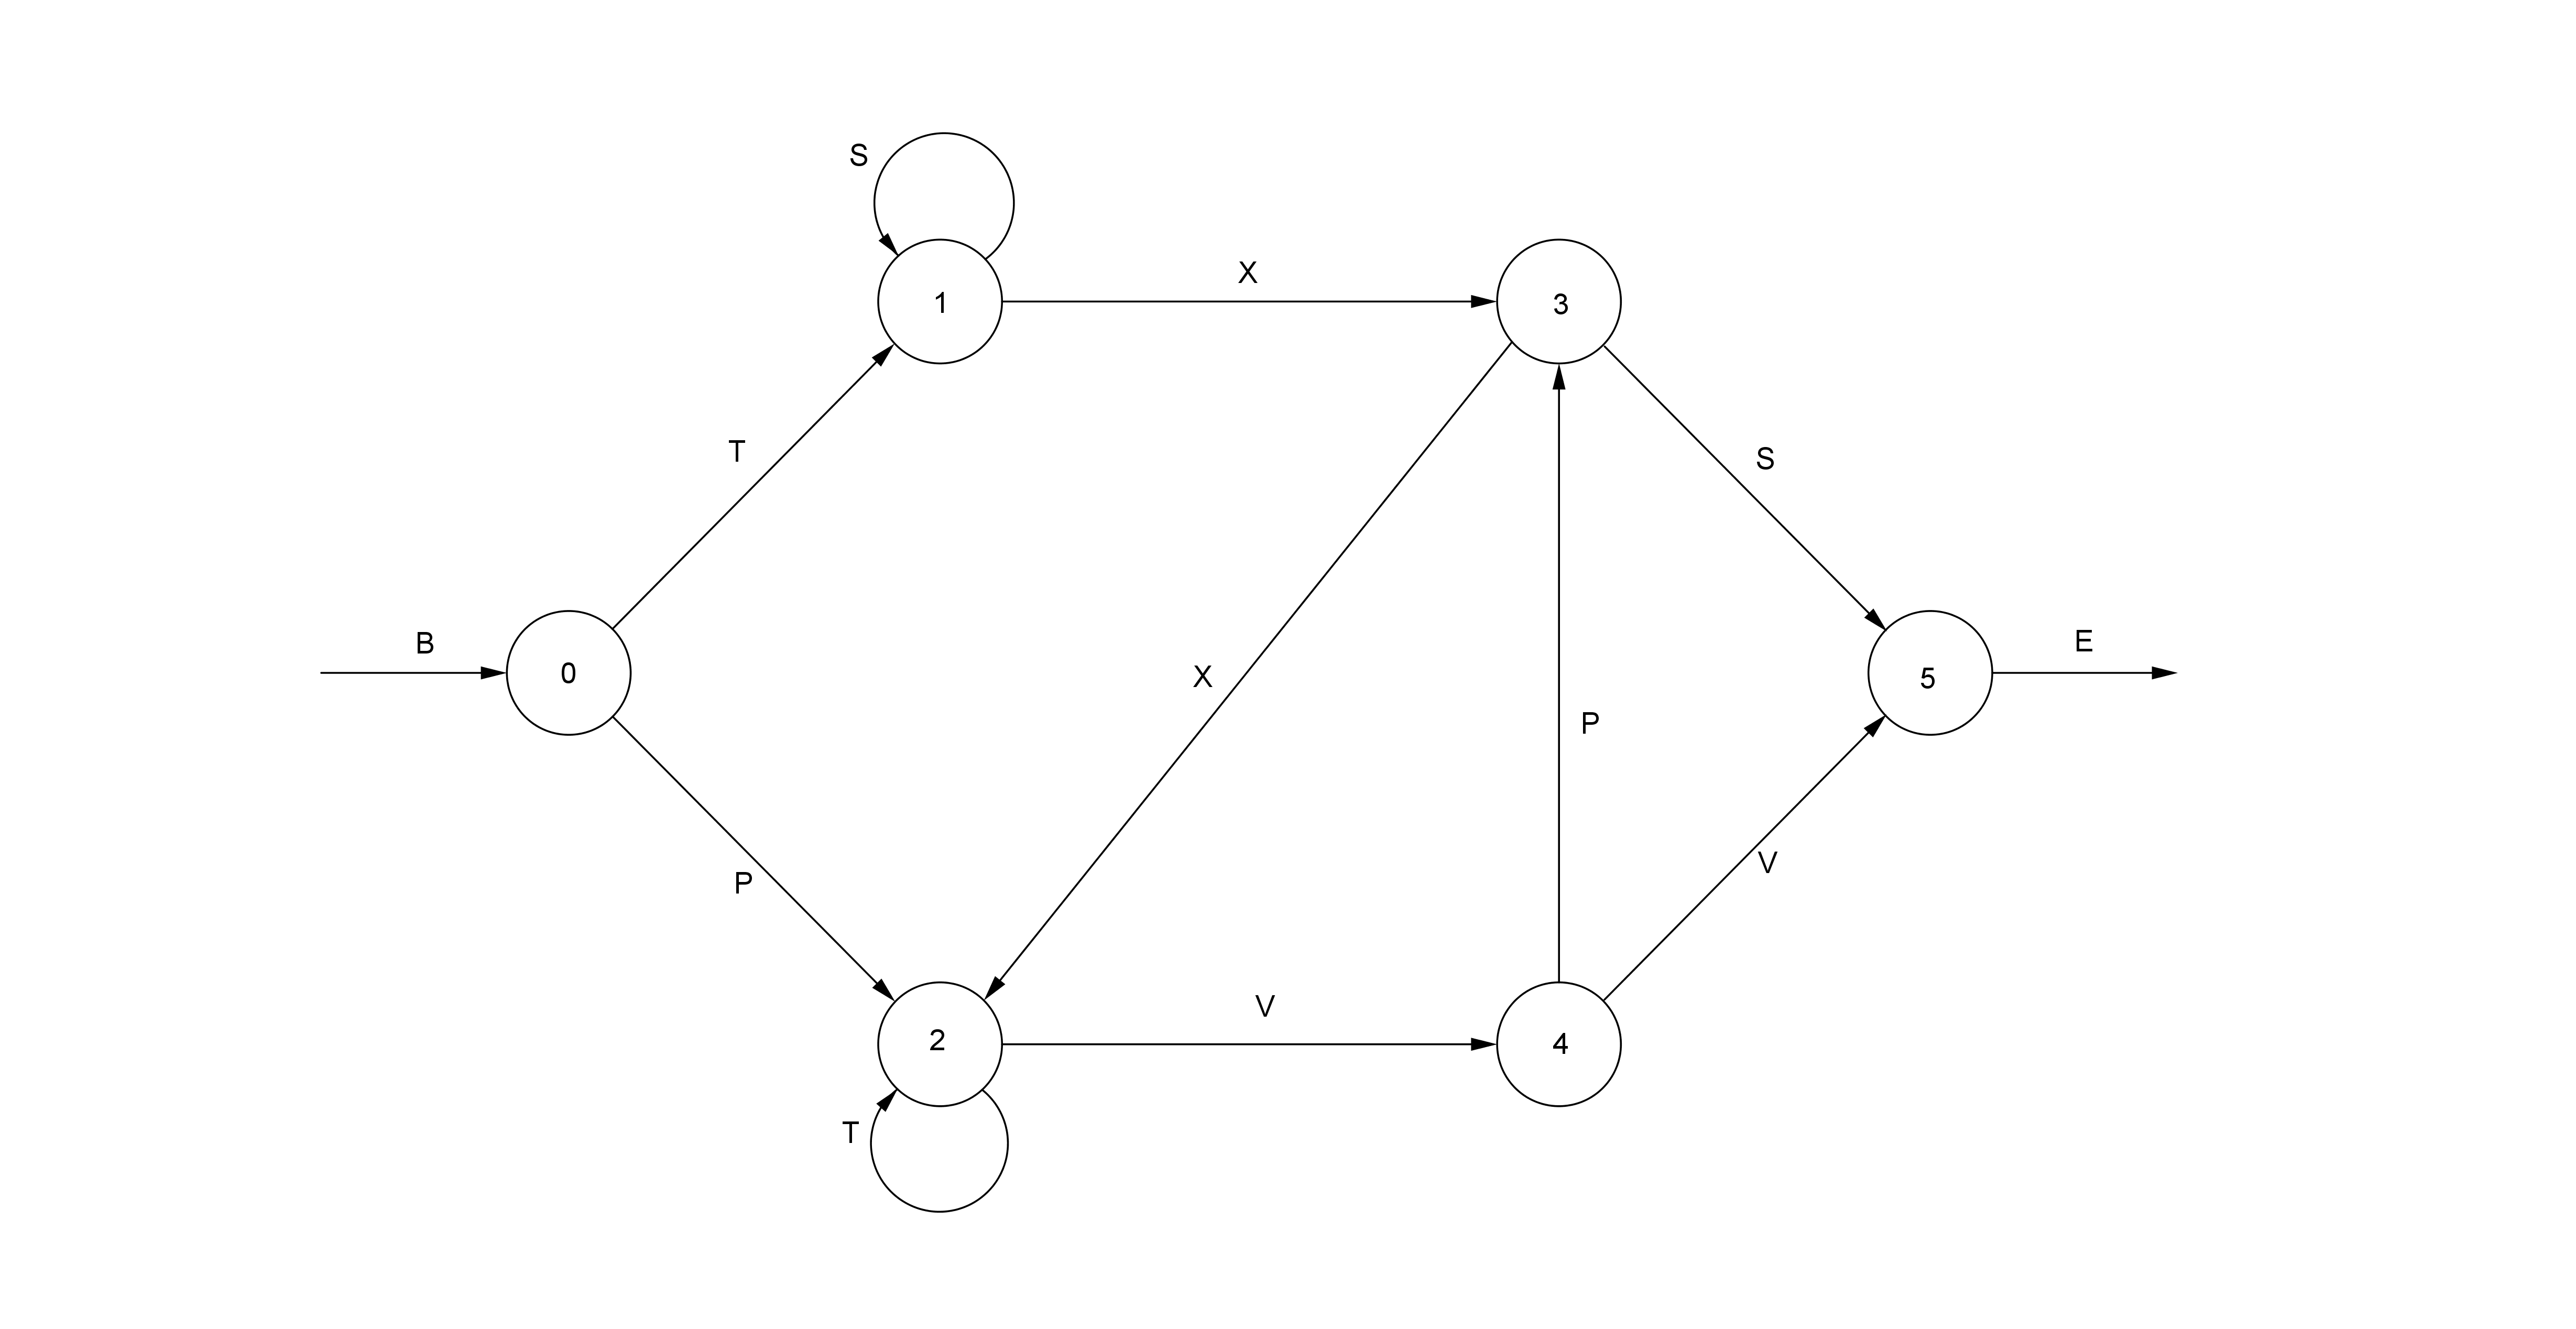
\includegraphics[scale=0.3]{images/reber_simple.png}
\caption{Automate reconnaissant la grammaire de Reber simple}
\label{Grammaire de Reber simple}
\end{center}
\end{figure}

A l'aide de cette automate, nous générerons deux ensembles de mots respectivement afin d'entraîner et de tester notre futur réseau. L'objectif du réseau sera alors d'apprendre cette grammaire afin de prédire les caractères possibles après un caractère donné.

L'étape suivante consistera à tester les algorithmes sur l'apprentissage de la grammaire de Reber symmétrique présentée sur la figure \ref{Grammaire de Reber symétrique}.  
\begin{figure}[h!]
\begin{center}
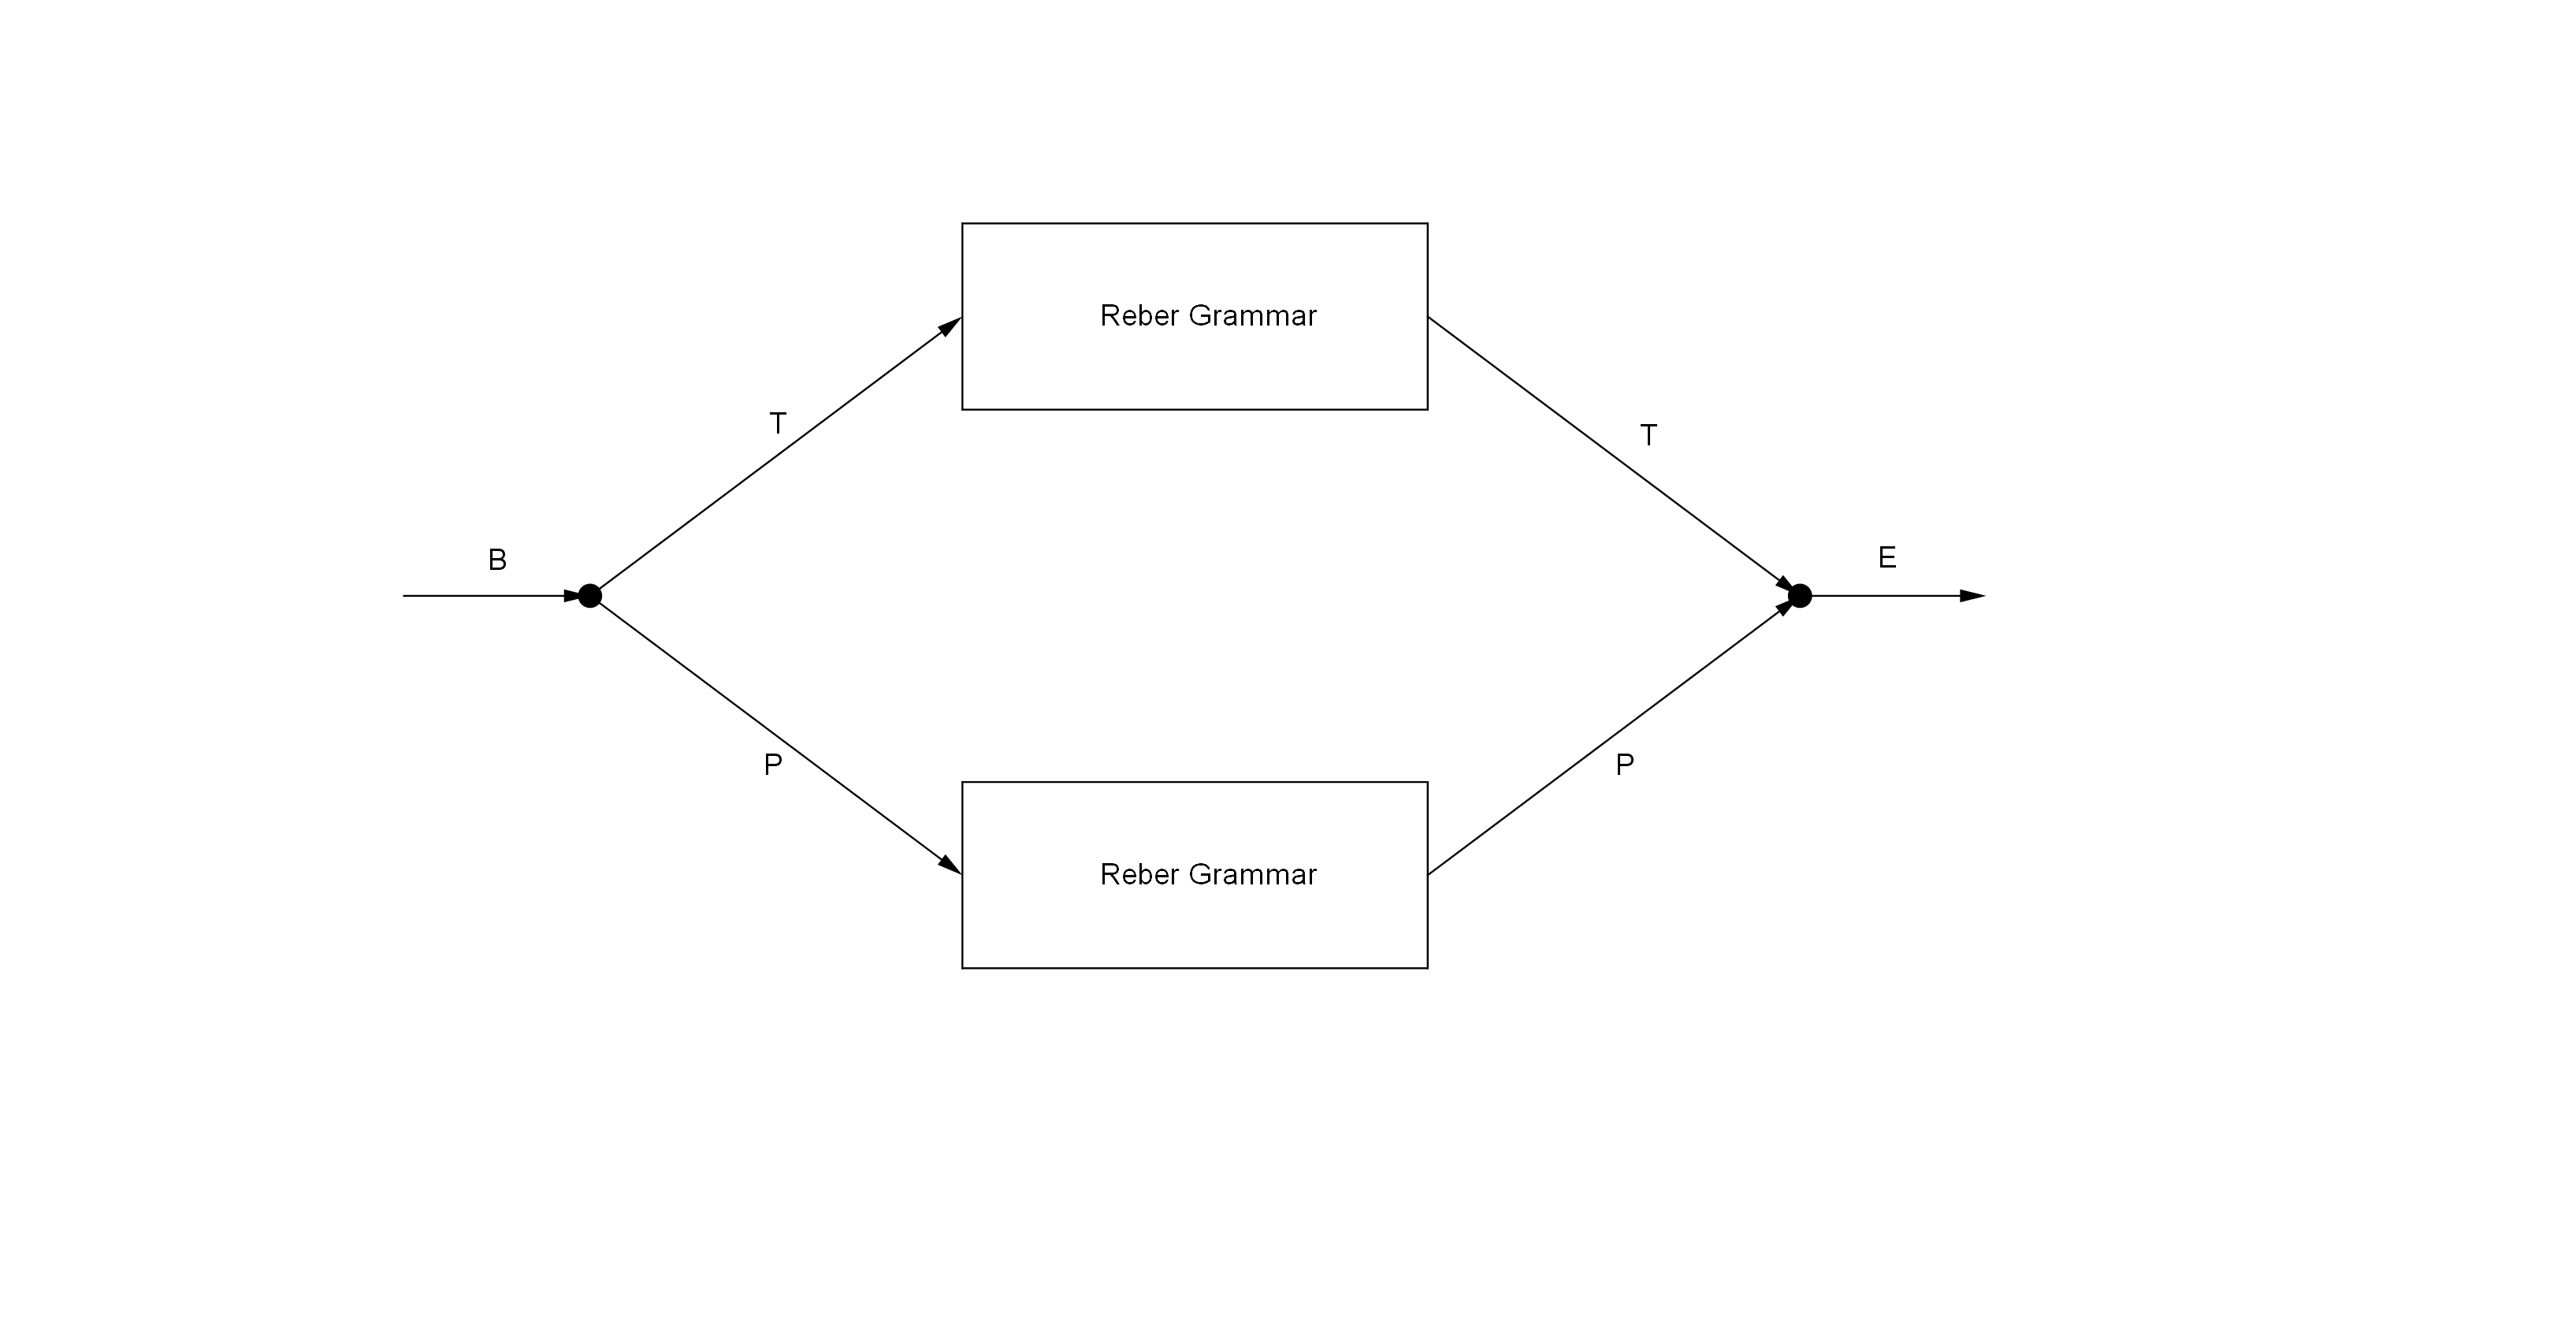
\includegraphics[scale=0.5]{images/reber_symmetrique.png}
\caption{Automate reconnaissant la grammaire de Reber symmétrique}
\label{Grammaire de Reber symmétrique}
\end{center}
\end{figure}

Dans cette situation, le réseau devra être capable de se souvenir d'un état passé (T ou P) afin de prédire le nouvel état (T ou P). Cet état passé pourra être plus ou moins lointain en fonction de la taille de la grammaire de Reber insérée au milieu. 

\section{Comparaison des deux algorithmes}

\section{Problème des dépendances temporelles}